% Metódy inžinierskej práce

\documentclass[10pt,twoside,slovak,a4paper]{article}

\usepackage[slovak]{babel}
%\usepackage[T1]{fontenc}
\usepackage[IL2]{fontenc} 
\usepackage[utf8]{inputenc}
\usepackage{graphicx}
\usepackage{url}
\usepackage{hyperref}
\usepackage{cite}


\pagestyle{headings}

\title{Gamifikácia ako nástroj motivácie v športoch

\author{Matej Drienovský\\[2pt]
	{\small Slovenská technická univerzita v Bratislave}\\
	{\small Fakulta informatiky a informačných technológií}\\
	{\small \texttt{xdrienovskym2@stuba.sk}}
	}

\date{\small 19. september 2022}
\thanks{Semestrálny projekt v predmete Metódy inžinierskej práce, ak. rok 2022/23, vedenie: Ing. Igor Stupavský}} 


\begin{document}

\maketitle

\begin{abstract}

Hlavným cieľom tohto článku je vniesť viac svetla do aspektov
gamifikácie. Najmä
v športovom kontexte. Vysvetlenie a oboznámenie, s pojmom gamifikácia. Jej účinok na
ľudskú psychiku. Jej základné využitie v rôznych športových aplikáciách, cez rôzne možnosti
napredovania pomocou levelov, získavania ocenení, spĺňania vopred určených cieľov,
porovnávania svojich výkonov s ďalšími použivateľmi aplikácie. Vplyv gamifikácie na športový
výkon, pomôcka k napredovaniu oproti ostatným. Prvky gamifikácie, a ako nás motivujú. Použitie aplikácií pri konkrétnych športoch, napríklad pri tvorbe zápasov
(matchmaking).
\end{abstract}


\section{Úvod}
Veľké množstvo ľudí hľadá aktivitu na vyplnenie voľného času, odreagovanie sa od práce, školy a podobne. Vo väčšine prípadov ich to zavedie k športu. 
Vďaka rozmachu informačnokomunikačných technológií sa mobilné zariadenia a senzory stali pevnou súčasťou každodenného života.
V dnešnej dobe je všetko realizované prostredníctvom aplikácií v smartphonoch. 
Môžme predpokladať, že ľudia používajú aj športové aplikácie \ref{aplikácie}, ktoré ich motivujú k lepším výkonom alebo umožnia lepšie sledovanie pokroku.\ref{gamifikacia v športoch} Aplikácie zbierajú dáta zo senzorov v zariadení a následne ich vedia vyhodnotiť.
Princípy aplikácií, ktoré nám uľachčia tvorbu zápasov \ref{Matchmaking} pri turnajoch a iných športových podujatiach.\cite{Effect_of_gamification-Framework}


\newpage
\section{Gamifikácia} \label{gamifikácia}

\begin{figure*}[tbh]
Gamifikácia je aplikácia herných dizajnových prvkov a herných princípov v neherných kontextoch. Môže sa tiež definovať ako súbor aktivít a procesov na riešenie problémov pomocou alebo za použitia charakteristík herných prvkov. Gamifikácia bežne využíva herné dizajnové
prvky pre zlepšenie produktivity organizácie, učenie, crowdsourcing, nábor a hodnotenie zamestnancov, fyzické cvičenie, dopravné priestupky,voličská apatia,a viac. Zbierka výskumov o gamifikácii ukazuje, že väčšina štúdií o gamifikácii zistila, že má pozitívne účinky na jednotlivcov.\cite{Gamification-Framework}


\subsection{Motivácia} 

Ako bolo zmienené, princípy gamifikácie motivujú ľudí k častejšiemu používaniu aplikácie a dávajú impulzy k dosiahnutiu cieľov. Tieto princípy tu budú vysvetlené podrobnejšie. 
\label{prvky} Prvky gamifikácie sa delia do troch kategórií :
\begin{itemize}
  \item {Komponenty}
  \item {Mechanické}
  \item {Dynamické}
\end{itemize}
Komponenty sú základné prvky, ktoré sa používajú pre každý iný prvok vysokej úrovne. Hlavné komponenty
\begin{itemize}
  \item {Body}
  \item {Odznaky}
  \item {Rebríčky}
\end{itemize}

    
Na základe modelu aplikácie Hook (Liu Li, 2016) \cite{Improving_motivation-Framework} poskytujú športové aplikácie oznámenia v súvislosti s plánovaným tréningom. Účelom notifikácii ktoré sú prítomné v aplikáciach je aby použivateľ dostal  upozornenie, že priateľ práve absolvoval tréning, otvoril aplikáciu, vykonal nejakú činnosť ako napríklad zablahoželal mu. Hlavným cieľom každej aplikácii je , aby používateľ sledoval aktivity ostatných použivateľov a budoval si kontakty s inými športovcami.

\end{figure*}
\newpage
\section{Gamifikácia v športoch} \label{gamifikacia v športoch}
\subsection{aplikácie} \label{aplikácie}

Gamifikačné prvky \ref{prvky} v športových aplikáciách sú kľúčovými prvkami na zmenu správania používateľov. Vo všeobecnosti sú aplikácie založené na spätnej väzbe a odmenách (napr. Strava, Nike+ Run, Runkeeper). Existujú však aplikácie, ktoré majú trochu iný prístup. Zombies Run, bežec vidí na obrazovke, kde sú zombies, aby vedel, ktorým smerom má bežať, aby ho zombie nechytili. Ďalším príkladom je Spotify, aplikácia na streamovanie hudby, ktorá má funkciu výberu hudby v rámci daného žánru, ktorá zodpovedá tempu behu používateľa. Na základe myšlienky hudby poskytuje aplikácia Rock My Run vybrané skladby, ktoré zodpovedajú tepovej frekvencii a krokom športovca. Počas športovej aktivity sú najčastejšie používanými hernými prvkami okamžitá spätná väzba a sledovanie postupu. Aplikácie majú vo všeobecnosti zjednodušené používateľské rozhranie, zatiaľ čo športovec sleduje tréning, aby používateľovi poskytli najdôležitejšie údaje a trendy (napr. rýchlosť, vzdialenosť, polohu). Ak používateľ vytvoril trasu, ktorú má počas tréningu sledovať, zobrazuje sa ukazovateľ pokroku. V službe Strava je možnosť zapnúť funkciu živého segmentu, ktorá športovcovi umožňuje vidieť štatistiky rovnako, ako keby tam boli všetci ostatní pretekári. Takmer ako vo videohre.\cite{Gamification_in_sport_apps-Framework}
Ako už bolo spomenuté, po absolvovaní tréningu sú v týchto aplikáciách najsilnejšie spätné väzby a mechanizmy odmeňovania. Od skúsenostných bodov, cez Fuel Score Nike až po trofeje a rôzne druhy meraní sa používajú na poskytnutie presnej spätnej väzby o tréningu. Tieto prvky pomáhajú pochopiť a zvýrazniť kľúčové body tréningu, napr. najrýchlejšie kolo, osobný rekord, najdlhší tréning.
Niektoré aplikácie odmeňujú používateľov udeľovaním odznakov, ak splnia určitú výzvu. Výzvy môžu fungovať ako spúšťač pre používateľov pridaním časového limitu a cieľa na dokončenie. Niekedy sa tieto výzvy týkajú skutočných udalostí, ako je Tour de France alebo Mount Everest, napr. zdolanie výšky Mount Everestu bicyklom alebo behom a získanie odznaku. Tieto udalosti môžu poskytnúť príbeh tréningu, čím ho robia zaujímavejším a pútavejším pre použivateľa. Športovec sa zžije s príbehom a bude sa snažiť športovať viac a viac. Zozbierané odmeny, odznaky sa zvyčajne vystavujú na na úvodnej strane konta použivateľa alebo v špecialnej sekcii na to určenej. Vystavené odznaky a trofeje sa vystavujú verejne, takže si ich môžu ostatní použivatelia, priatelia prehliadnuť.\cite{Effect_of_gamification-Framework}

\subsection{Matchmaking} \label{Matchmaking}
Matchmaking je spojenie dvoch a viac ľudí (hráčov) napríklad do jednej hernej relácie. Vedci skúmali ako ovplyvní zabudovanie matchmakingu a gamifikačných prvkov do aplikácií zameranej na tvorbu tenisových zápasov. Táto aplikácia obsahovala jednoduché menu v ktorom si použivateľ vedel zvoliť miesto zápasu, svoju úroveň v tenise a pohlavie. Na základe zadaných údajov aplikácia vytriedila možnosti a možných súperov. Použivateľov aplikácia spojila a dohodli si presný termín a konkrétne miesto konania.
Cieľovou skupinou boli zamestnanci spoločnosti Ericsson Nikola Tesla. Mnohí z týchto zamestnancov sa venujú nejakému druhu rekreačných športových aktivít, takže by to mala byť dobrá vzorka pre výskum. 
\newpage
Jedna z otázok prieskumu bola zameraná na otázku či si respondenti myslia, že používanie tejto aplikácie sa prejaví tak, že v budúcnosti budú viac hrať tenis. \cite{Improving_motivation-Framework} Výsledkom prieskumu je znázornení jednoduchým diagramom. Kde mierne prevažuje možnosť áno. 

\hfill \break 
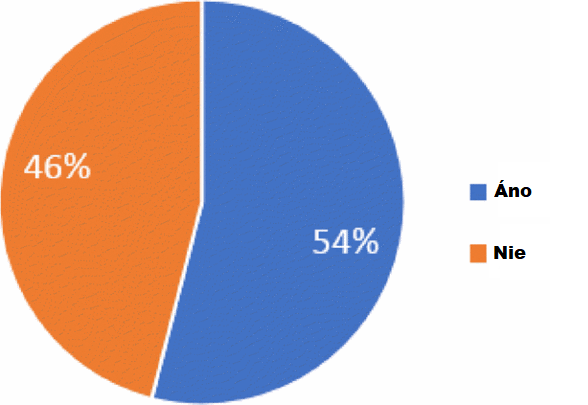
\includegraphics[scale =0.6]{graf_tenis.png}


\subsection{Prieskum} \label{Prieskum}
Podľa prieskumov, ktoré boli zamerané na zistenie učinkov jednotlivých herných mechanizmov na človeka, a ktoré herné mechanizmy majú najlepší účinok na človeka. V prvej časti prieskumu bolo cieľom zistiť, aký druh športu vykonávaju a  rozdeliť ľudí do dvoch kategórií, profesionáli a ostaní športovci. \ref{Výsledok} Kedže, profesionál je skúsenejší a dokáže potrobnejšie chápať a skúmať údaje z tréningu. V druhom bloku sa zisťovala pravidelnosť športovania na základe troch parametrov. Prvým bolo priemerné trvanie jedného cvičenia, druhým aspektom bol priemerný počet tréningov za týždeň. Tretia otázka bola zameraná na kategorizáciu intenzity aktivity športovania. Na základe týchto troch kritérií sa vypočítalo celkové skóre v rozmedzí od 0 do 126. \cite{Effect_of_gamification-Framework} V treťom sektore sa pýtali ľudí aký šport a s akou pravidelnosťou ho vykonávajú. Bola to podstatná informácia, ktorú bolo potrebné vedieť, aby bolo možné prepojiť údaje ku konkrétnym športom. Štvrtý blok bol zameraný na otázky o aplikáciach ktoré využívaju počas tréningov. Zisťovala sa užitočnosť, spokojnosť a úroveň ich odporúčania.\ref{Výsledok aplikácie} Piaty blok prieskumu bol zameraný na meranie charakteristík prvkov gamifikácie v športových aplikáciach. Toto meranie bolo uskutočnené pomocou 21 výrokov v súvislosti s rôznymi scenárami v športe. Respondent mal ohodnotiť výrok na štvorstupňovej Likertovej škále od silne nesúhlasím po silne súhlasím.
Posledný blok tvorili demografické otázky, vek, najvyšší stupeň ukončenej školy.\cite{Effect_of_gamification-Framework}
\newpage
\subsection{Výsledok} \label{Výsledok}
Bicyklovanie bolo najvyššie v rebríčku medzi každodenne používanými športmi, beh a fitness boli na ďaľších dvoch miestach. Z nasledujúceho grafu vyplýva, že bicykel ľudia využívajú nielen na športovanie ale aj ako dopravný prostriedok.\cite{Effect_of_gamification-Framework}

\hfill \break
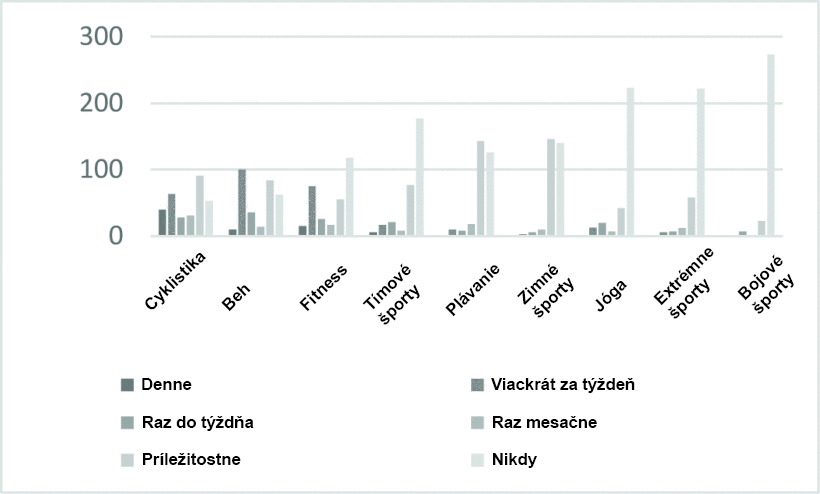
\includegraphics[scale =0.4]{obrazok3.png}
\hfill \break
\label{Výsledok aplikácie}
Z ďaľšej časti prieskumu je vidieť, že z hodnotených aplikácií najlepšie obstála aplikácia Polar a za ňou nasledovali aplikácie Garmin a Strava. Polar aj Garmin predávajú profesionálne športové produkty ako napríklad hodinky, športové náramky a to môže byť dôvod prečo sú ich aplikácie sú najlepšie hodnotenými.

\hfill \break
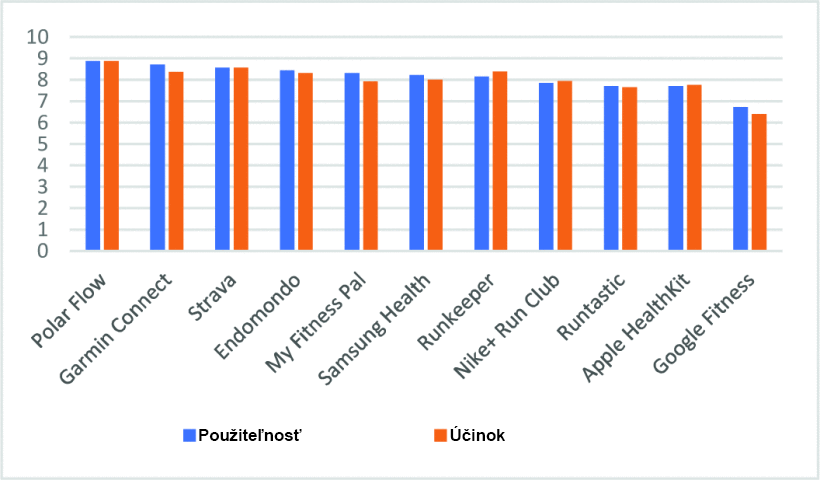
\includegraphics[scale =0.5]{obrazok1.png}

 Zaujímavosť, ktorú prieskum ukázal bolo to, že odmeny po každom tréningu boli najmenej dôležité. Ďalším výsledkom, ktorý si vyžaduje pozornosť, je 10. miesto, otázka o vplyve priateľov používajúcich aplikáciu. Ak priateľ používa určitú aplikáciu, nebude to pre športovca dôležitý prvok, ktorý by mal brať do úvahy.\cite{Effect_of_gamification-Framework}
\hfill \break
\begin{table}[!ht]
    \centering
    \begin{tabular}{|l|l|l|l|}
    \hline
        ~ & Hodnotenie funkcií v aplikáciach podľa prieskumu & ~ & ~ \\ \hline
        ~ & Najväčší účinok & ~ & Menší účinok \\ \hline
        1 & Funkcie zadarmo & 7 & Hlásenia počas cvičenia \\ \hline
        2 & Vzhľad výsledku z cvičenia & 8 & Kompatibilita \\ \hline
        3 & Stabilita aplikácie & 9 & Vzhľad aplikácie \\ \hline
        4 & Jednoduchosť používania & 10 & Priatelia používajúci aplikáciu \\ \hline
        5 & Presnosť jednotlivých meraní & 11 & Náučne vlastnosti \\ \hline
        6 & Prispôsobenie aplikácie & 12 & Hodnotenia za cvičenie \\ \hline
    \end{tabular}
\end{table}
\newpage
Ďaľší a zároveň posledný blok bol zameraný na sledovanie herných prvkov v aplikáciach. Výsledky naznačujú, že spomedzi herných prvkov testovaných v štúdii majú na účastníkov najväčší vplyv okamžitá spätná väzba a ukazovatele pokroku.
Okamžitá spätná väzba v športe je jedným z najzákladnejších herných prvkov, ktoré sa používajú, keďže počas tréningu sa poskytujú informácie o aktuálnom stave a po skončení tréningu sa zobrazia zachytené údaje. Z vlastnej skúsenosti môžem povedať, že túto funkciu využívam najčastejšie. Priebežné lišty sú prospešné hlavne počas tréningov, keď sa v nich vizuálne zobrazuje pokrok napríklad trvanie a vzdialenosť. Športovec tak získava informácie o tom, koľko úsilia je potrebné vynaložiť na dokončenie tréningu.\cite{Effect_of_gamification-Framework} 
Levely alebo nové rekordy sa stali najpozitívnejšie hodnoteným prvkom.
\section{Zhrnutie}
Gamifikácia sa stala každodennou súčasťou nášho života. Čoraz viac aplikácií, firiem a pod. využíva jej princípy. Pre väčší prehľad je dobré ich poznať. Spoločnosti tlačia gamifikáciu do svojich produktov gamifikácia sa teší čoraz väčšej popularite. Množstvo obrovských korporácií ju využíva k zlepšniu dosahov a zvýšeniu obľúbenosti ich produktov. 
\section{Reakcia na témy z prednášok}
\subsection{Tranzistor}
Tranzistor je trojvrstvová polovodičová súčiastka, ktorá sa skladá z troch vrstiev polovodičového materiálu. \cite{Tranzistory-Framework} Vnútorná vrstva, ktorá má opačný typ nevlastnej vodivosti ako vonkajšie vrstvy, sa nazýva báza. Vonkajšie vrstvy sú emitor a kolektor. Poznáme tranzistory PNP a NPN. 
\hfill
\break
Využitie : 
\begin{itemize}
  \item {Spracovanie signálu (zosiľňovač)}
  \item {Realizácia logických obvodov ( AND, OR, NOT, NAND, XOR, ...)}
  \item {Pamäť}
\end{itemize}
Anglický matematik a logik George Boole zapísal výroky formulami ktoré sa algebraickými úpravami mohli upravovať , napr. zjednodušiť. Uľachčilo to tvorbu logických obvodov.\cite{Tranzistory2-Framework}

\subsection{Git}
Git je open source verzovací systém. Môžeme ho ovládať cez príkazoví riadok alebo cez GUI pre Git. \cite{Git-Framework} Git ukladá celú históriu projektu na všetkých zariadeniach, kde bol daný repozitár stiahnutý.
Git príkazy: 
\begin{itemize}
  \item {git init}
  \item {git status}
  \item {git add .}

\end{itemize}

 \subsection{Prezentovanie}
 Prezentácia by mala byť plynulá a veľmi dôležitá vec je vyhýbať sa slovám ako ehm, hm a pod. K publiku by sme mali hovoriť dostatočne nahlas, a používať svoj hlas ako nástroj. Nástroj, ktorým, dokážeme zaujať publikum, zdôrazniť dôležité časti. Potrebné je samozrejme naštudovať si o čom budeme prednášať. Nikdy celý text nečítame. Je to neprofesionálne a nie moc pekné pre publikum. Odporúčam zapojiť počas prejavu aj obecenstvo. Vytvoríte priamy kontakt s obecenstvom. Tento spôsob sa odporúča pri konferenciách a prednáškach ale je to neprípustné pri obhajobe projektov. Ďaľšou pomôckou pri prejave môže byť spoznanie obecenstva a výklad mierne prispôsobiť, pokojne aj na mieste.

\section{Diagram práce na článku}
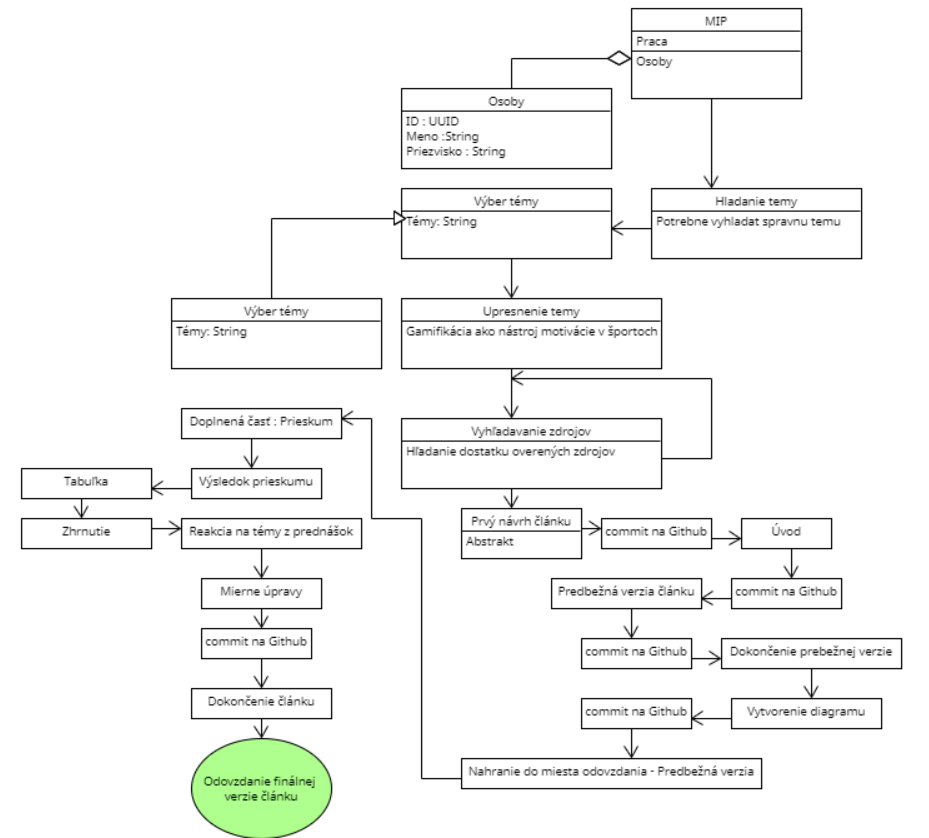
\includegraphics[scale =0.7]{diagram.png}
\newpage
\bibliography{literatura}
\bibliographystyle{abbrv}
\end{document}
